%%%%%%%%%%%%%%%%%%%%%%%%%%%%%%%%%%%%%%%%%%%%%%%%%%%%%%%%%%%%%%%%%%%%
%% I, the copyright holder of this work, release this work into the
%% public domain. This applies worldwide. In some countries this may
%% not be legally possible; if so: I grant anyone the right to use
%% this work for any purpose, without any conditions, unless such
%% conditions are required by law.
%%%%%%%%%%%%%%%%%%%%%%%%%%%%%%%%%%%%%%%%%%%%%%%%%%%%%%%%%%%%%%%%%%%%

% This theme was based on fibeamer theme 
% If you found any bugs please contact @karlosos
% This repository is hosted on github https://github.com/karlosos/zut-fibeamer/

\documentclass{beamer}
\usetheme[faculty=wi]{fibeamer}
\usepackage[utf8]{inputenc}
\usepackage[
  main=polish,
  polish
]{babel}

\title{Introdução a disciplina}
\subtitle{Tópicos especiais em Sistemas}
\author{Prof. Juliana Costa Silva - juliana.silva@up.edu.br}

\usepackage{ragged2e}  % `\justifying` text
\usepackage{booktabs}  % Tables
\usepackage{tabularx}
\usepackage{tikz}      % Diagrams
\usetikzlibrary{calc, shapes, backgrounds}
\usepackage{amsmath, amssymb}
\usepackage{url}       % `\url`s
\usepackage{listings}  % Code listings
\frenchspacing
\begin{document}

%------------------------------------------------------------------------
  \frame[c]{\maketitle}
  \AtBeginSection[]{% Print an outline at the beginning of sections
    \begin{frame}<beamer>
      \frametitle{O que veremos hoje}
      \tableofcontents
    \end{frame}}
%------------------------------------------------------------------------
    \section{Introdução}
    \subsection{Sobre a disciplina}
    \begin{frame}{Plano de Aulas}
      \framesubtitle{Disponível no BlackBoard}%
      
      \begin{itemize}
            \item 1 Bimestre: 5 pontos (2 trabalhos  -  3 prova)
            \item 2 Bimestre: 5 pontos (2 trabalhos - 3 prova)
            \item Uma atividade por aula a contar da semana 2 (percentual de entrega defina a nota de trabalho);
       \end{itemize}
     \end{frame}
%------------------------------------------------------------------------
    \begin{frame}[label=lists]{Ferramentas e tecnologias}
      \begin{columns}[onlytextwidth]
        \column{.5\textwidth}
          \begin{itemize}
            \item NodeJS \textcolor{gray}{(instalar até a próxima aula)}
            \item VSCode \textcolor{gray}{(ou outra IDE da preferência do aluno)}
            \item AngularJS 
          \end{itemize}
        \column{.5\textwidth}
            
\includegraphics[width=55mm]{resources/aula1_4.png}
      \end{columns}
    \end{frame}
%------------------------------------------------------------------------
    \subsection{NodeJS}
    \begin{frame}[label=simmonshall]{NodeJS}

      \begin{block}{O que é?}
        Um \alert{JS Runtime Enviroment}: Ambiente de execução Javascript.
      \end{block}
      \begin{exampleblock}{O que ele não é?}
        Não é um framework, nem uma linguagem de programação.
      \end{exampleblock}
      \begin{alertblock}{Pra que serve??}
        Para desenvolvimento de aplicações Javascript, backend, frontend, APIs, microserviços.
      \end{alertblock}
    \end{frame}
%------------------------------------------------------------------------
    \begin{frame}[label=proof]{Vantagens NodeJS}
	\begin{itemize}
	\item Rápido;
	\item Alta escalabilidade
	\item Ecosistema muito grande (NPM)
	\item Empresas como: Netflix e PayPal utilizam.
	\item Javascript (front, back mobile... tudo)
	\end{itemize}
    \end{frame}
    
       %------------------------------------------------------------------------
    \begin{frame}[label=lists]{Funcionamento NodeJS}
            
\includegraphics[width=90mm]{resources/aula1_5.png}\\
            \tiny{\textbf{Fonte:} \cite{ich2021}}
    \end{frame}
    %------------------------------------------------------------------------
    \begin{frame}[label=lists]{Funcionamento NodeJS}
      \begin{columns}[onlytextwidth]
        \column{.5\textwidth}
          \alert{Node.js} é escrito não apenas em Javascript, mas também em $C++$ e Javascript. \\
          Para operar corretamente, depende de muitas bibliotecas. \\
          No entanto, V8 e LIBUV são duas dependências mais importantes que tratam da maioria das operações do Node.js.

        \column{.5\textwidth}
            
\includegraphics[width=55mm]{resources/aula1_6.png}\\
            \tiny{\textbf{Fonte:} \cite{ich2021}}

      \end{columns}
    \end{frame}
    
 %------------------------------------------------------------------------
    \begin{frame}[label=lists]{Funcionamento V8]}
      \begin{columns}[onlytextwidth]
        \column{.5\textwidth}
          Node.js é construído no motor V8 do Google. Este é um mecanismo de javascript rápido. \\
          O motor V8 tem o papel de converter o código javascript em código de máquina que o computador entende.\\
          \vspace{0.5cm}
	O Node.js não entende o código javascript que escrevemos sem o V8.
        \column{.5\textwidth}
            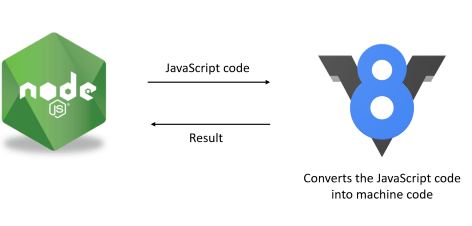
\includegraphics[width=65mm]{resources/aula1_7.png}\\
            \tiny{\textbf{Fonte:} \cite{ich2021}}

      \end{columns}
    \end{frame}
    
  %------------------------------------------------------------------------
    \begin{frame}[label=lists]{Entrada e saída Assíncrona}
     \framesubtitle{O que é isso?}%

          LIBUV é outra  dependência do Node.js. Esta dependência permite ao Node o acesso ao sistema operacional da máquina, rede, sistema de arquivos e muito mais.\\
          \vspace{0.5cm}
          LIBUV é uma biblioteca de código aberto com um forte foco em E / S assíncrona (entrada-saída). LIBUV é escrito em C ++. Além de focar na E / S assíncrona, LIBUV também implementa dois recursos importantes que são o loop de eventos e o pool de threads.          
          
    \end{frame}
    
 %------------------------------------------------------------------------
    \begin{frame}[label=lists]{Loops e Eventos}
     \framesubtitle{O que é isso?}%
      \begin{columns}[onlytextwidth]
        \column{.5\textwidth}
         Quando usamos Node.js em um computador, significa que há um processo de nó em execução nesse computador. 
         \\
	Nesse processo, o Node.js é executado em uma única thread. \\
	O que é importante entender aqui, é o fato de que o nó roda em apenas um thread, por exemplo, se tivermos 4 tarefas diferentes, então todas essas quatro tarefas acontecerão em uma única thread.          
          \vspace{0.5cm}
	
        \column{.5\textwidth}
            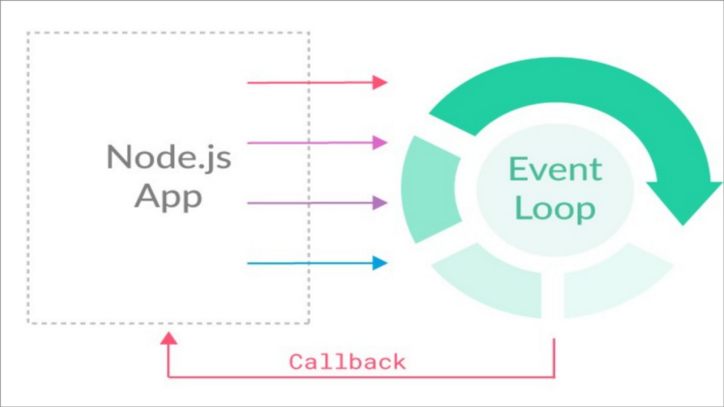
\includegraphics[width=65mm]{resources/aula1_8.png}\\
            \tiny{\textbf{Fonte:} \cite{ich2021}}

      \end{columns}
    \end{frame}
%------------------------------------------------------------------------
   \subsection{Referências}
    \begin{frame}{Referências}%[allowframebreaks]
\frametitle{Referências}
\small
\begin{center}
\tiny
\bibliographystyle{apalike}
\bibliography{ref_aula}
\end{center}
\end{frame}
\end{document}
